\part{Design Goals}
\frame{\partpage}

\begin{frame}{Intro}
	\begin{itemize}
		\item As a designer it is important to have sort of intent
		\item It is important to think of what kind of response you want from your audience
		\item Its also important to document your design decisions
	\end{itemize}
\end{frame}

\begin{frame}{Design Document (GGD)}
	\begin{itemize}
		\item This traditionally documented all the decisions made by the designer in one place
		\item The act of writing this forced the designer to think through their process
		\item One major issue, is that these docs became monolithic and were not read by the team
		\item There is no standard format for Design Docs
	\end{itemize}
\end{frame}

\begin{frame}{Evolution of the Design Doc}
	\begin{itemize}
		\item Design docs would be kept up to date when the design shifted
		\item Gradually these docs were moved to Wiki's or Google Docs
		\item This allows the GGD to be updated and collaborated on
	\end{itemize}
\end{frame}

\begin{frame}{Suggest GGD Structure}
	\begin{itemize}
		\item \textbf{Taken from Game Design Workshop Chapter 14 Pg 459 - 464} 
		\item Overview and Vision Statement
		\item Audience, platform, and marketing
		\item Gameplay
		\item Characters (if applicable)
		\item Story (if applicable)
		\item World (if applicable)
		\item Media List
	\end{itemize}
\end{frame}

\begin{frame}{Design Pillars}
	\begin{itemize}
		\item Something about your game that everything should revolve around
		\item Establish once the your are in production
		\item Better for larger games
		\item Traditionally this is focused on mechanics but try to think about emotions you want at the core of your game
	\end{itemize}
\end{frame}

\begin{frame}{Audience/Player Experience Goals}
	\begin{itemize}
		\item Less rigid than Design Pillars
		\item You should focus on the emotional journey you want the player to experience
		\item This should inform your design process at all times
		\item If a feature detracts from this experience then cut it
	\end{itemize}
\end{frame}

\begin{frame}{Game Design Macro}
	\begin{itemize}
		\item Monolithic Design Docs are not very useful
		\item No-one in the team reads them
		\item Document is slow to evolve
		\item Game Design Macro attempts to capture the high level design 
	\end{itemize}
\end{frame}

\begin{frame}{Game Design Macro}
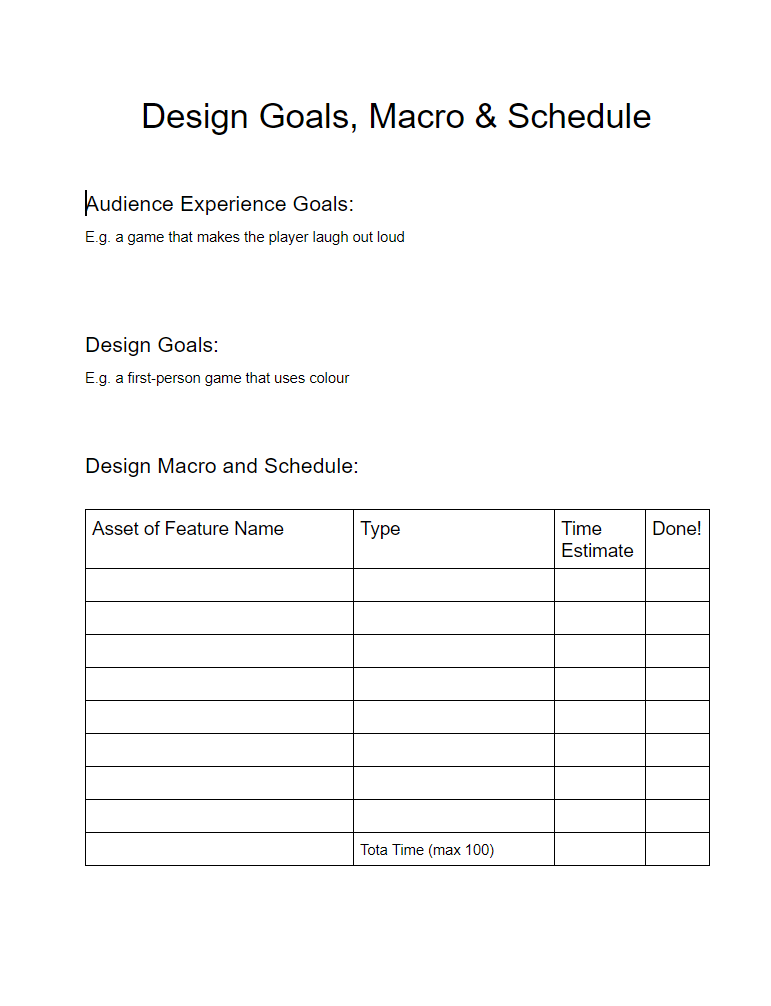
\includegraphics[width=0.7\textwidth,height=0.7\textheight]{game_design_macro}
\end{frame}

\begin{frame}{One Page Designs}
	\begin{itemize}
		\item First described by Stone Librande (Riot Games) 
		\item Instead of writing a monolithic Design Doc
		\item You write a series of one page design docs which detail some aspect of the game
		\item This could be a map, a visual description of the combat, relationship between characters
	\end{itemize}
\end{frame}

\begin{frame}{One Page Designs}
	\begin{center}
		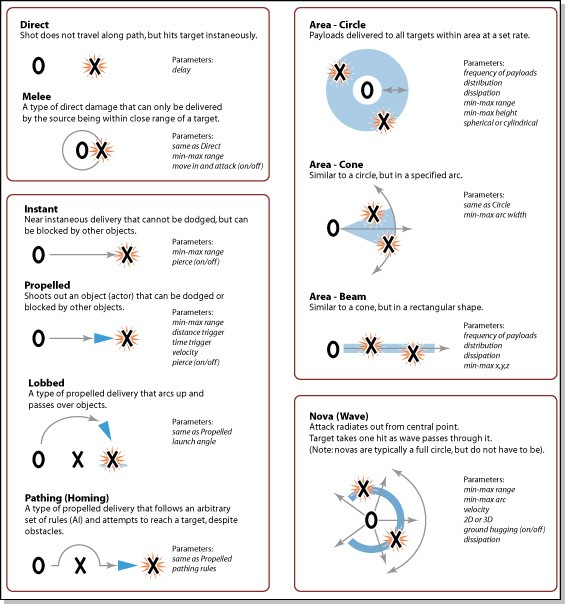
\includegraphics[width=0.7\textwidth,height=0.7\textheight]{combat_diagram}
	\end{center}
\end{frame}

\begin{frame}{One Page Designs}
	\begin{center}
		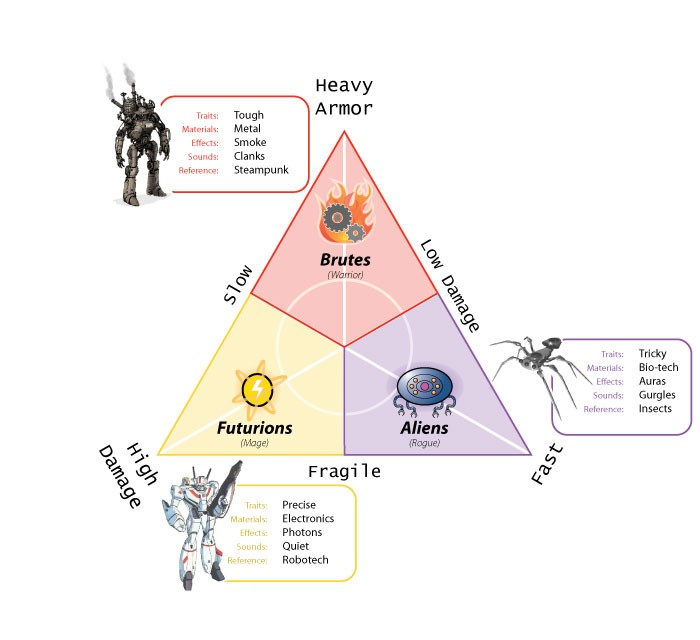
\includegraphics[width=0.7\textwidth,height=0.7\textheight]{unit_diagram}
	\end{center}
\end{frame}

\begin{frame}{One Page Design Template}
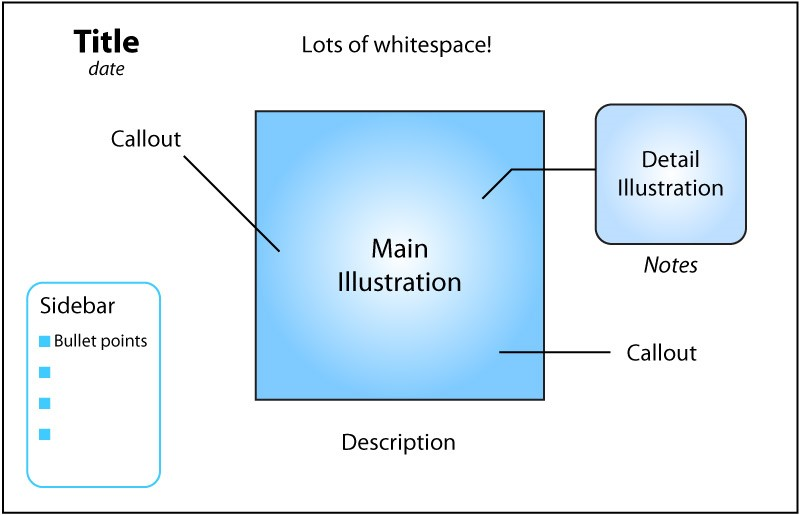
\includegraphics[width=1.0\textwidth]{one_page_design_template}
\end{frame}

\begin{frame}{One Page Design Benefits}
\begin{itemize}
	\item Forces a complete understanding of the game
	\item Forces a concise design
	\item Highlights relationships
	\item Aids problem solving
\end{itemize}

\end{frame}
